\documentclass[11pt]{article}
\usepackage[margin=1in]{geometry}
\usepackage[spanish]{babel}
\usepackage{fontspec}
\setmonofont{Menlo}
\usepackage{hyperref}
\usepackage{orcidlink}
\usepackage{graphicx}
\usepackage{tocloft}
\usepackage{fvextra}
\fvset{breaklines=true,breakanywhere=true,fontsize=\small}
\setlength{\emergencystretch}{2em}
\setlength{\cftsubsecnumwidth}{3.5em}

\title{p-adic GRN Suite\\\large Plataforma integral para análisis p-ádico de redes de regulación genética}
\author{
Jesús Rogelio Pérez-Buendía\,\orcidlink{0000-0002-7739-4779}
\and
Víctor Nopal-Coello\,\orcidlink{0000-0003-2608-3636}
\and
Yuriria Cortés-Poza\,\orcidlink{0000-0003-1856-9206}
}
\date{Periodo de desarrollo: 2023--2026}

\begin{document}
\maketitle

\begin{abstract}
Este documento presenta el software científico \emph{p-adic GRN Suite}, diseñado para el análisis p-ádico de redes de regulación genética en dinámica discreta finita. El software está organizado en tres partes funcionales: \textit{core} (métricas p-ádicas), \textit{search} (búsqueda/certificación de orderings) y \textit{viz} (visualización y reportes). El reporte reúne documentación funcional, manuales de uso, scripts de validación, código fuente, pruebas automatizadas, ejemplos de corridas con resultados reales y evidencia reproducible, además del estado actual del demo web institucional.
\end{abstract}

\tableofcontents
\newpage

\section{Introducción y alcance del software}
\emph{p-adic GRN Suite} es un software amplio y especializado para análisis p-ádico de redes de regulación genética. Su diseño es general para sistemas de dinámica discreta finita y su operación integra cálculo, búsqueda/certificación y visualización en un flujo científico reproducible. Este software consta de tres partes técnicas que se usan de forma coordinada en un mismo flujo de trabajo:
\begin{itemize}
  \item \textbf{core}: cálculo de métricas p-ádicas sobre dinámicas discretas finitas.
  \item \textbf{search}: búsqueda/certificación de orderings con estrategias computacionales.
  \item \textbf{viz}: visualización y comunicación reproducible de resultados.
\end{itemize}

Relación operacional de uso:
\begin{enumerate}
  \item Se define el sistema y se calculan métricas con \textit{core}.
  \item Se exploran/certifican orderings con \textit{search} usando el mismo marco matemático.
  \item Se generan figuras y salidas de reporte con \textit{viz}.
\end{enumerate}

Con este esquema, la suite mantiene coherencia científica y técnica, y documenta en un solo expediente todo el proceso de análisis.

\subsection*{Fundamentos teóricos y referencias}
Los fundamentos matemáticos del método están desarrollados en las siguientes referencias. Sobre esta base teórica, el software se reporta como plataforma de análisis computacional para redes regulatorias en dinámica discreta finita:
\begin{itemize}
  \item Pérez-Buendía, J. R.; Nopal-Coello, V. \emph{Hierarchical p-Adic Framework for Gene Regulatory Networks: Theory and Stability Analysis}. arXiv:2603.14097. Disponible en: \url{https://arxiv.org/abs/2603.14097}
  \item Pérez-Buendía, J. R.; Nopal-Coello, V.; Cortés-Poza, Y. \emph{Regulatory p-Adic Orderings from Stability in Gene Networks: Applications and Validation in Three Developmental Systems}. Zenodo, registro 19482987. Disponible en: \url{https://zenodo.org/records/19482987}
\end{itemize}

\section{Contribución científica verificable}
La \emph{p-adic GRN Suite} implementa de manera reproducible una metodología
computacional para el análisis matemático de redes de regulación genética en
dinámica discreta finita, articulando en un solo flujo tres capacidades
complementarias: cálculo de métricas p-ádicas, búsqueda/certificación de
orderings y visualización de resultados.

\subsection*{Funcionalidad que habilita}
La suite organiza en un mismo entorno de trabajo tres actividades centrales del
análisis p-ádico de dinámicas discretas: (i) cálculo de indicadores, (ii)
exploración de estructuras de ordenamiento y (iii) generación de salidas
interpretables para discusión científica. Esta integración fortalece la
coherencia metodológica y la reproducibilidad del flujo completo.

\subsection*{Novedad y aporte}
El aporte verificable de software consiste en operacionalizar, dentro de una
arquitectura modular y testeada, métodos p-ádicos de análisis de redes en
dinámica discreta finita para:
\begin{itemize}
  \item cuantificar comportamiento p-ádico por medio de \texttt{mu\_E},
  \texttt{mu\_A}, \texttt{mu\_I} y sus perfiles asociados;
  \item identificar orderings candidatos y certificarlos con estrategias
  computacionales (heurísticas y exhaustivas);
  \item generar artefactos de comunicación reproducibles para validación y
  reporte.
\end{itemize}

\subsection*{Evidencia reproducible incluida}
La contribución está respaldada por:
\begin{itemize}
  \item código fuente ejecutable y versionado en las tres partes del software;
  \item pruebas automatizadas y corridas de validación en cada módulo;
  \item ejemplos de corridas con salidas numéricas reales incluidas en este
  expediente;
  \item script maestro de validación integral para ejecutar la suite de forma
  unificada.
\end{itemize}

\section{Ventajas, necesidad y valor del software}
\subsection*{Necesidad científica y técnica}
El análisis de redes de regulación genética con enfoque p-ádico requiere
integrar, en un mismo flujo, cálculo matemático, exploración sistemática de
orderings y visualización interpretable de resultados. La suite proporciona
ese flujo integrado con estructura operativa y trazabilidad reproducible.

\subsection*{Ventajas principales}
\begin{itemize}
  \item Integra en un solo entorno operativo las tres etapas del análisis:
  \textit{core}, \textit{search} y \textit{viz}.
  \item Estandariza entradas, salidas y validaciones, fortaleciendo la
  consistencia de ejecución y la auditoría técnica.
  \item Permite combinar búsqueda heurística y certificación sistemática para
  estudiar orderings con criterio cuantitativo.
  \item Produce resultados verificables y comunicables mediante reportes,
  figuras y archivos de evidencia.
\end{itemize}

\subsection*{Aporte y valor para la comunidad}
El software aporta una infraestructura reproducible para llevar métodos p-ádicos
del plano teórico al análisis computacional aplicado. Su valor reside en hacer
operativo un flujo completo de trabajo, con trazabilidad de resultados y
documentación utilizable por personas investigadoras, estudiantes y equipos
técnicos en biología matemática y sistemas dinámicos discretos.

\subsection*{Uso reportado}
En este expediente se documenta su uso mediante corridas reproducibles, pruebas
automatizadas y validaciones integradas para las tres partes de la suite.
Asimismo, las referencias citadas en la introducción reportan su aplicación en
redes regulatorias de \textit{Arabidopsis thaliana}, \textit{Caenorhabditis
elegans} y \textit{Drosophila melanogaster}.
Su uso también se reporta en líneas de investigación activas para problemas
particulares de regulación genética y otros sistemas biológicos analizados por
equipos de investigación.

\section{Alcance operativo y condiciones de uso}
\subsection*{Alcance operativo}
La versión documentada corresponde a una suite científica funcional para análisis p-ádico de redes de regulación genética en dinámica discreta finita, con resultados reproducibles en línea de comandos, visualizaciones y evidencia formal en pruebas y archivos de salida.

\subsection*{Condiciones de uso reportadas}
\begin{itemize}
  \item El software incluye tres partes coordinadas: \textit{core},
  \textit{search} y \textit{viz}, integradas en un flujo único de trabajo.
  \item El demo web institucional proporciona interfaz de consulta, backend de
  verificación y guía de despliegue para uso demostrativo.
  \item Este expediente incorpora documentación técnica, manuales de usuario,
  ejemplos de corridas con resultados reales y scripts de validación.
  \item Los campos de DOI y enlaces oficiales se reportan con identificadores
  de referencia y se actualizan con los identificadores definitivos de
  publicación.
\end{itemize}

\section{Datos generales del software}
\begin{itemize}
  \item Nombre de software: \texttt{p-adic GRN Suite}
  \item Versión de integración documental: \texttt{1.0.0}
  \item Lenguaje principal: Python 3.10+
  \item Partes del software: \texttt{padic-grn-core}, \texttt{padic-grn-search}, \texttt{padic-grn-viz}
  \item DOI (Zenodo): \texttt{DOI\_ZENODO\_SUITE}
\end{itemize}

\subsection{Enlaces oficiales}
\begin{itemize}
  \item Repositorio GitHub (suite): \texttt{URL\_GITHUB\_SUITE}
  \item Release GitHub (versión actual): \texttt{URL\_GITHUB\_RELEASE}
  \item Registro Zenodo (suite): \texttt{URL\_ZENODO\_SUITE}
  \item DOI de versión (snapshot Zenodo): \texttt{DOI\_VERSION}
  \item DOI conceptual (todas las versiones): \texttt{DOI\_CONCEPTUAL}
\end{itemize}

\subsection{Actualización de enlaces}
Los identificadores de referencia se reemplazan con enlaces y DOI oficiales una vez emitidos por los repositorios institucionales correspondientes.

\section{Manual de usuario de la suite}
\VerbatimInput{MANUAL-USUARIO.md}

\section{Ejemplos de corridas de la suite}
\subsection{Resumen claro de corridas con resultados reales}
Esta subsección sintetiza corridas reales verificables para lectura rápida del
evaluador, incluyendo entrada, comando, salida principal e interpretación.

\subsubsection*{Corrida 1: scoring con \textit{core} (toy, $p=2$, $N=2$)}
\begin{itemize}
  \item Entrada: \texttt{padic-grn-core/examples/transitions\_p2\_n2\_identity.csv}
  \item Comando: \texttt{pgcore-score-ordering ... 2 2 "0 1" --output-json}
  \item Evidencia de salida: \texttt{core\_scores\_p2.json} (carpeta de evidencia de corridas)
  \item Resultado real: \texttt{mu\_E=0}, \texttt{mu\_A=0}, \texttt{mu\_I=4}
  \item Interpretación: en este caso de referencia, el comportamiento reportado
  es de indiferencia p-ádica predominante (\texttt{mu\_I} máximo relativo).
\end{itemize}

\subsubsection*{Corrida 2: búsqueda genética con \textit{search}}
\begin{itemize}
  \item Objetivo: \texttt{minimize\_mu\_E}
  \item Evidencia de salida: \texttt{search\_ga\_p2.json} (carpeta de evidencia de corridas)
  \item Resultado real: método GA con PMX, \texttt{best\_ordering=[1,0]},
  \texttt{best\_fitness=0}, \texttt{evaluations=2}
  \item Resultado real de métricas: \texttt{mu\_E=0}, \texttt{mu\_A=0},
  \texttt{mu\_I=4}
\end{itemize}

\subsubsection*{Corrida 3: certificación exacta con \textit{search}}
\begin{itemize}
  \item Evidencias: \texttt{search\_bbmin\_p2.json} y \texttt{search\_bbmax\_p2.json}
  \item Métodos reales reportados: branch-and-bound con cota parcial para
  minimización de \texttt{mu\_E} y backtracking exacto para maximización de
  \texttt{mu\_A}.
  \item Resultado real en el caso toy: \texttt{best\_ordering=[0,1]} y
  \texttt{best\_fitness=0} para ambos objetivos.
\end{itemize}

\subsubsection*{Corrida 4: validación global de suite}
\begin{itemize}
  \item Script maestro: \texttt{RUN-ALL-VALIDATIONS.sh}
  \item Alcance: ejecución de validaciones de \textit{core}, \textit{search} y
  \textit{viz} en una sola corrida.
  \item Evidencia complementaria: archivos \texttt{validacion\_*\_pytest.txt} en
  cada módulo.
\end{itemize}

\subsection{Documento detallado de ejemplos}
\VerbatimInput{EJEMPLOS-CORRIDAS.md}

\subsection{Correos electrónicos oficiales de autores}
\begin{itemize}
  \item Jesús Rogelio Pérez-Buendía: \texttt{rogelio.perez@cimat.mx}
  \item Víctor Nopal-Coello: \texttt{victor\_nopal@uaeh.edu.mx}
  \item Yuriria Cortés-Poza: \texttt{yuriria.cortes@iimas.unam.mx}
\end{itemize}

\subsection{Financiamiento}
\begin{itemize}
  \item Modelos matemáticos y computacionales no convencionales para el estudio y análisis de problemas relevantes en Biología, CF 2019/217367.
\end{itemize}

\subsection{Autoría oficial consolidada}
La autoría, ORCID y correos institucionales presentados en este expediente
corresponden a la versión oficial del software y se reportan de forma
consistente en portada, metadatos de paquete y archivos de citación.

\section{Sección I: Módulo core (métricas p-ádicas)}
\subsection{README}
\VerbatimInput{padic-grn-core/README.md}
\subsection{Manual de usuario}
\VerbatimInput{padic-grn-core/MANUAL-USUARIO.md}
\subsection{Manual técnico}
\VerbatimInput{padic-grn-core/MANUAL-TECNICO.md}
\subsection{Configuración de paquete}
\VerbatimInput{padic-grn-core/pyproject.toml}
\subsection{Cita académica}
\VerbatimInput{padic-grn-core/CITATION.cff}
\subsection{Licencia}
\VerbatimInput{padic-grn-core/LICENSE}
\subsection{Configuración de pruebas}
\VerbatimInput{padic-grn-core/pytest.ini}
\subsection{Código fuente}
\VerbatimInput{padic-grn-core/src/padic_grn_core/__init__.py}
\VerbatimInput{padic-grn-core/src/padic_grn_core/cli.py}
\VerbatimInput{padic-grn-core/src/padic_grn_core/adapters.py}
\VerbatimInput{padic-grn-core/tools/validate_expected_values.py}
\subsection{Pruebas y ejemplos}
\VerbatimInput{padic-grn-core/tests/test_smoke.py}
\VerbatimInput{padic-grn-core/tests/test_adapters.py}
\VerbatimInput{padic-grn-core/examples/transitions_p2_n2_identity.csv}
\VerbatimInput{padic-grn-core/examples/transitions_p3_n2_identity.csv}
\VerbatimInput{padic-grn-core/examples/orderings_n2.csv}
\subsection{Evidencia de validación}
\VerbatimInput{padic-grn-core/registro_autor/validacion_core_pytest.txt}
\VerbatimInput{../registro-dossier/06_evidencia_corridas/core_scores_p2.json}
\VerbatimInput{../registro-dossier/06_evidencia_corridas/core_scores_p3.json}
\VerbatimInput{../registro-dossier/06_evidencia_corridas/core_batch_p2.csv}

\section{Sección II: Módulo search (búsqueda/certificación)}
\subsection{Programas de optimización incluidos}
\begin{itemize}
  \item \texttt{pgsearch-ga}: búsqueda heurística con objetivo seleccionable
  (minimizar \texttt{mu\_E} o maximizar \texttt{mu\_A}).
  \item \texttt{pgsearch-bb-min-muE}: branch-and-bound/backtracking exacto para minimizar \texttt{mu\_E}, con poda por cota parcial cuando está disponible.
  \item \texttt{pgsearch-bb-max-muA}: búsqueda exacta por backtracking para maximizar \texttt{mu\_A}.
\end{itemize}

\subsection{README}
\VerbatimInput{padic-grn-search/README.md}
\subsection{Manual de usuario}
\VerbatimInput{padic-grn-search/MANUAL-USUARIO.md}
\subsection{Manual técnico}
\VerbatimInput{padic-grn-search/MANUAL-TECNICO.md}
\subsection{Configuración de paquete}
\VerbatimInput{padic-grn-search/pyproject.toml}
\subsection{Cita académica}
\VerbatimInput{padic-grn-search/CITATION.cff}
\subsection{Licencia}
\VerbatimInput{padic-grn-search/LICENSE}
\subsection{Configuración de pruebas}
\VerbatimInput{padic-grn-search/pytest.ini}
\subsection{Código fuente}
\VerbatimInput{padic-grn-search/src/padic_grn_search/__init__.py}
\VerbatimInput{padic-grn-search/src/padic_grn_search/cli.py}
\VerbatimInput{padic-grn-search/src/padic_grn_search/engine.py}
\subsection{Pruebas}
\VerbatimInput{padic-grn-search/tests/test_smoke.py}
\VerbatimInput{padic-grn-search/tests/test_engine.py}
\subsection{Evidencia de validación}
\VerbatimInput{padic-grn-search/registro_autor/validacion_search_pytest.txt}
\VerbatimInput{../registro-dossier/06_evidencia_corridas/search_ga_p2.json}
\VerbatimInput{../registro-dossier/06_evidencia_corridas/search_bbmin_p2.json}
\VerbatimInput{../registro-dossier/06_evidencia_corridas/search_bbmax_p2.json}

\section{Sección III: Módulo viz (visualización/reportes)}
\subsection{README}
\VerbatimInput{padic-grn-viz/README.md}
\subsection{Manual de usuario}
\VerbatimInput{padic-grn-viz/MANUAL-USUARIO.md}
\subsection{Manual técnico}
\VerbatimInput{padic-grn-viz/MANUAL-TECNICO.md}
\subsection{Configuración de paquete}
\VerbatimInput{padic-grn-viz/pyproject.toml}
\subsection{Cita académica}
\VerbatimInput{padic-grn-viz/CITATION.cff}
\subsection{Licencia}
\VerbatimInput{padic-grn-viz/LICENSE}
\subsection{Configuración de pruebas}
\VerbatimInput{padic-grn-viz/pytest.ini}
\subsection{Código fuente}
\VerbatimInput{padic-grn-viz/src/padic_grn_viz/__init__.py}
\VerbatimInput{padic-grn-viz/src/padic_grn_viz/cli.py}
\VerbatimInput{padic-grn-viz/src/padic_grn_viz/engine.py}
\subsection{Pruebas}
\VerbatimInput{padic-grn-viz/tests/test_smoke.py}
\VerbatimInput{padic-grn-viz/tests/test_engine.py}
\subsection{Evidencia de validación}
\VerbatimInput{padic-grn-viz/registro_autor/validacion_viz_pytest.txt}

\section{Scripts globales y corridas de integración}
\subsection{Script maestro de validación}
\VerbatimInput{RUN-ALL-VALIDATIONS.sh}

\subsection{Evidencia de casos de estudio}
\VerbatimInput{../Paper-II.v3.2/results/ATHALIANA_OPTIMA_SUMMARY.md}
\VerbatimInput{../Paper-II.v3.2/supplementary/data/RECALCULO_MU_OPTIMOS_TABLAS.md}
\VerbatimInput{../Paper-II.v3.2/supplementary/data/VERIFICACION_SIMETRIAS_Y_NUMEROS.md}

\section{Applets y UI web reportada}
\subsection{Estado actual y alcance}
El demo web institucional comprende dos applets HTML autocontenidos (sin dependencias de servidor externo), un backend mínimo de referencia y guía de despliegue. Los applets implementan la metodología p-ádica completa directamente en el navegador, incluyendo: clasificación E/A/I de bolas p-ádicas, visualización fractal animada con rotación progresiva por nivel, grafo de transición funcional con detección de ciclos, análisis polinomial ANF mediante transformada de Möbius, búsqueda interactiva de orderings óptimos y soporte para redes personalizadas vía CSV.

\subsection{Applet principal: p-adic Ball Structure — GRN Animation}
\texttt{padic-balls-animation.html} — applet autocontenido que implementa:
\begin{itemize}
  \item Clasificación E/A/I de bolas p-ádicas con visualización fractal animada y rotación progresiva por nivel de anidamiento.
  \item Grafo de transición funcional $x \to f(x)$ con detección automática de ciclos y estructura $\rho$ (pestaña \emph{Transition graph}).
  \item Análisis polinomial en Forma Normal Algebraica (ANF) mediante transformada de Möbius sobre $\mathbb{F}_2^N$ — $O(N \cdot 2^N)$ — con detección de identidades, simetrías y factorizaciones (pestaña \emph{Polynomial structure}).
  \item Búsqueda de ordering óptimo: exhaustiva, algoritmo genético (GA) y branch-and-bound.
  \item Soporte para redes personalizadas vía CSV (formato vectores de bits o enteros decimales).
  \item Redes incluidas: \textit{C. elegans} ($N=8, p=2$), \textit{Drosophila melanogaster} ($N=6, p=2$), \textit{A. thaliana} ($N=13, p=2$).
\end{itemize}

\VerbatimInput{web-demo-institucional/padic-balls-animation.html}

\subsection{Applet secundario: p-adic GRN Demo}
\texttt{padic-grn-demo.html} — applet de visualización de perfil de métricas $\mu_E$, $\mu_A$, $\mu_I$ por nivel de resolución, con tabla de resultados y gráfica de perfil comparativo.

\VerbatimInput{web-demo-institucional/padic-grn-demo.html}

\subsection{Datos de ejemplo para redes personalizadas}
Archivos CSV de ejemplo incluidos para prueba y demostración del soporte de redes arbitrarias:
\VerbatimInput{web-demo-institucional/boolean_N4_example.csv}
\VerbatimInput{web-demo-institucional/z2mod16_N4_p2.csv}

\subsection{Registro de cambios del demo web}
\VerbatimInput{web-demo-institucional/CHANGELOG.md}

\subsection{README del demo web}
\VerbatimInput{web-demo-institucional/README.md}
\subsection{Backend de referencia}
\VerbatimInput{web-demo-institucional/backend/app.py}
\subsection{Guía de despliegue}
\VerbatimInput{web-demo-institucional/docs/DEPLOY.md}

\subsection{Capturas de pantalla del demo}
\begin{figure}[htbp]
  \centering
  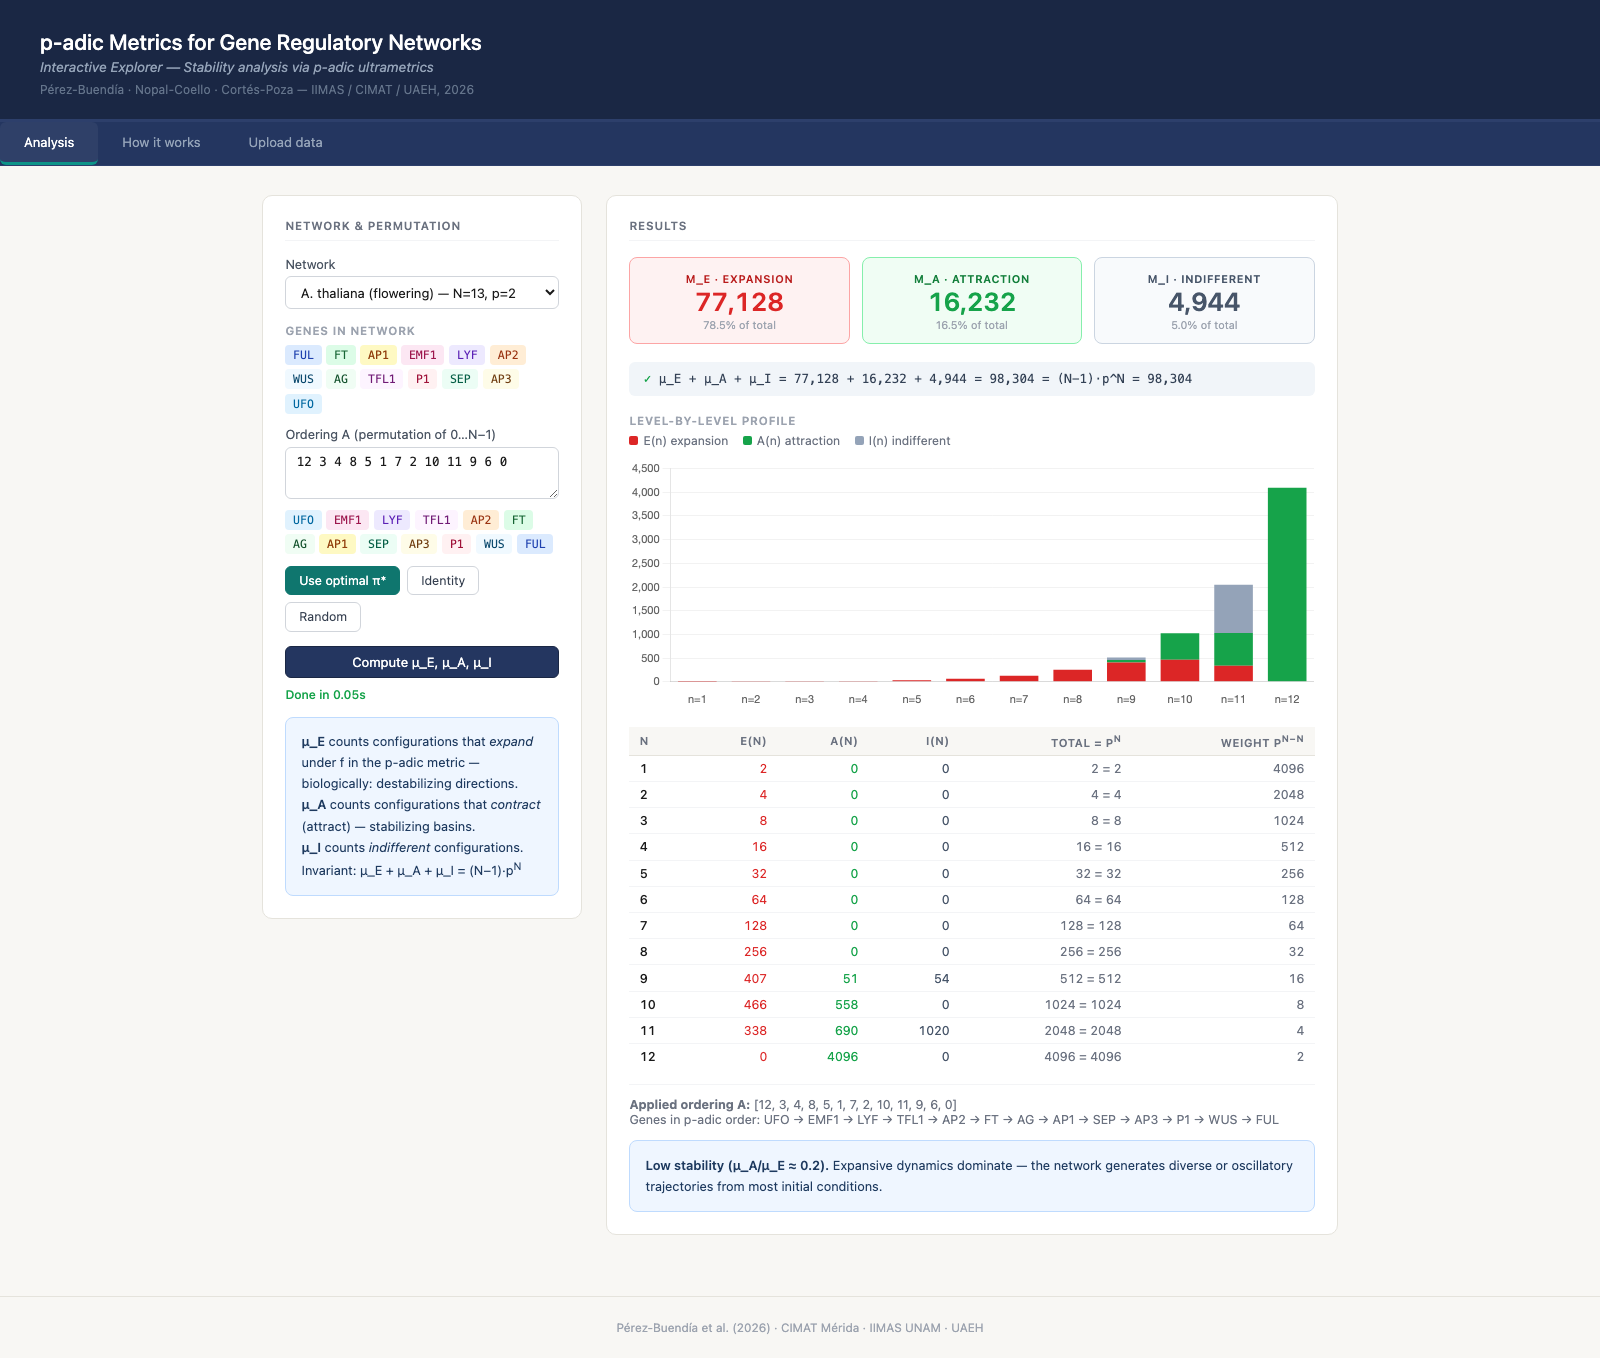
\includegraphics[width=\textwidth]{web-demo-institucional/screenshots/registro-padic-grn-demo-running-desktop.png}
  \caption{Demo \texttt{padic-grn-demo.html} en ejecución real (escritorio): cálculo de \texttt{mu\_E}, \texttt{mu\_A}, \texttt{mu\_I}, gráfica de perfil y tabla de resultados.}
\end{figure}

\begin{figure}[htbp]
  \centering
  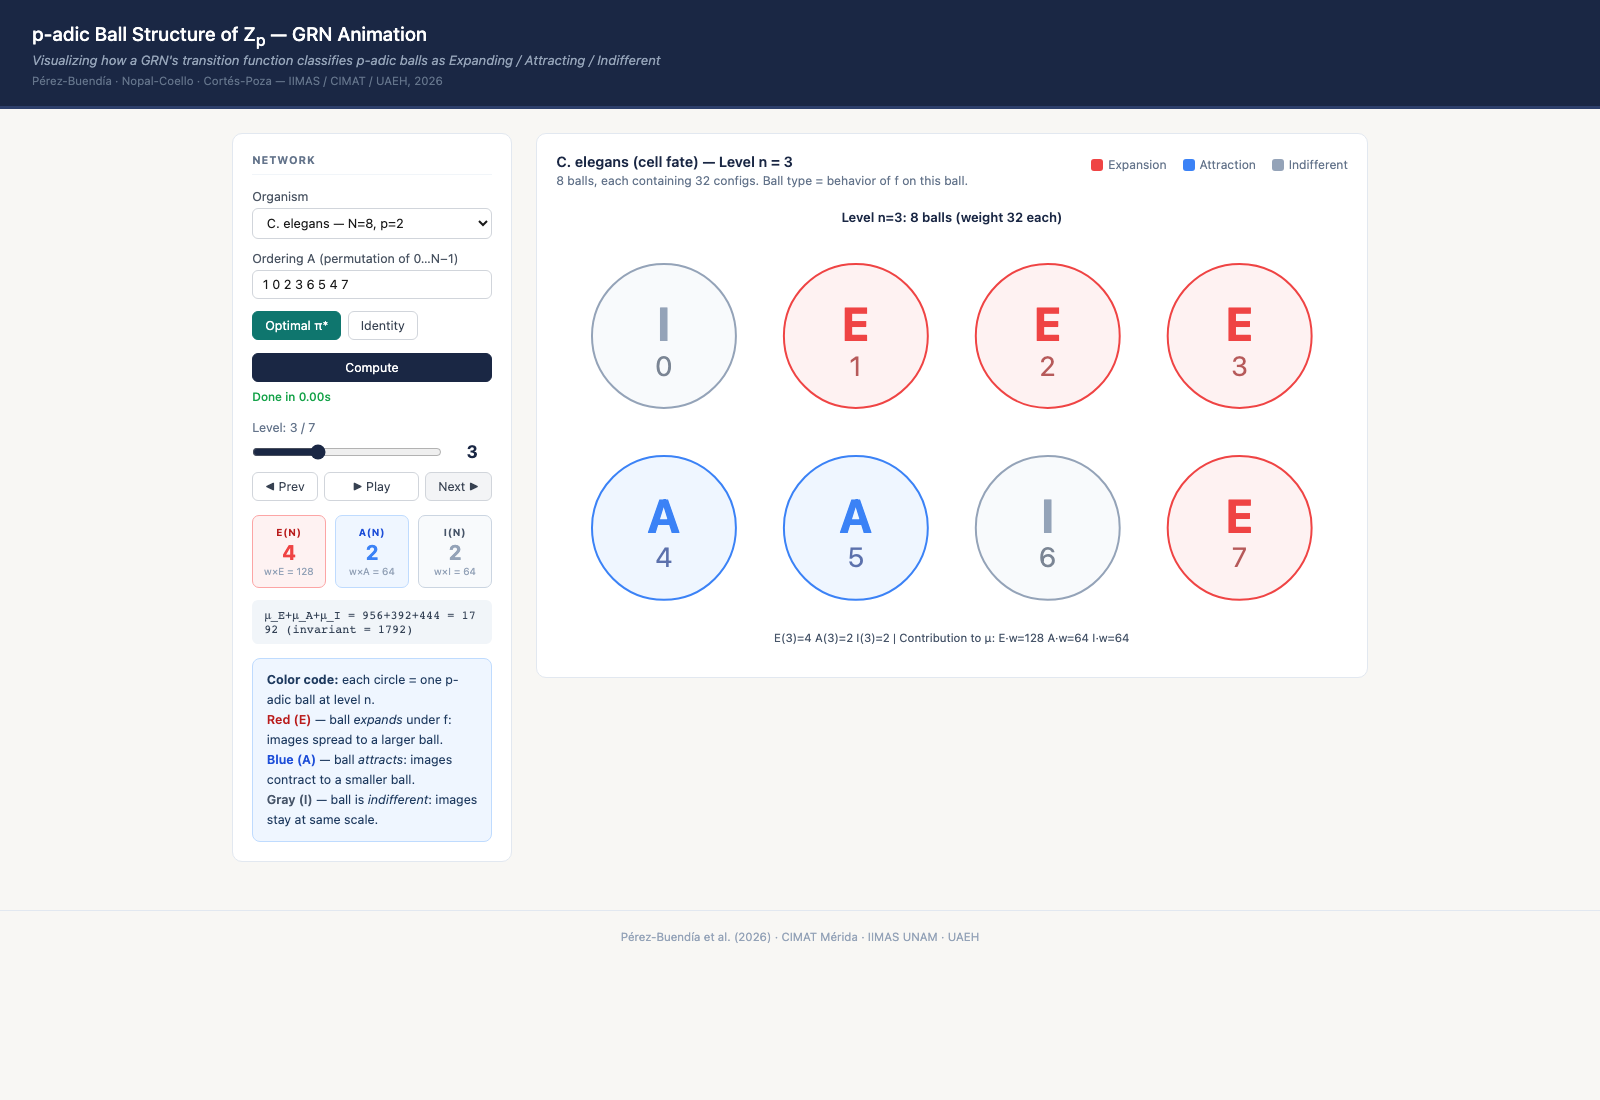
\includegraphics[width=\textwidth]{web-demo-institucional/screenshots/registro-padic-balls-running-desktop.png}
  \caption{Demo \texttt{padic-balls-animation.html} en ejecución real (escritorio): clasificación de bolas p-ádicas y navegación por niveles.}
\end{figure}

\begin{figure}[htbp]
  \centering
  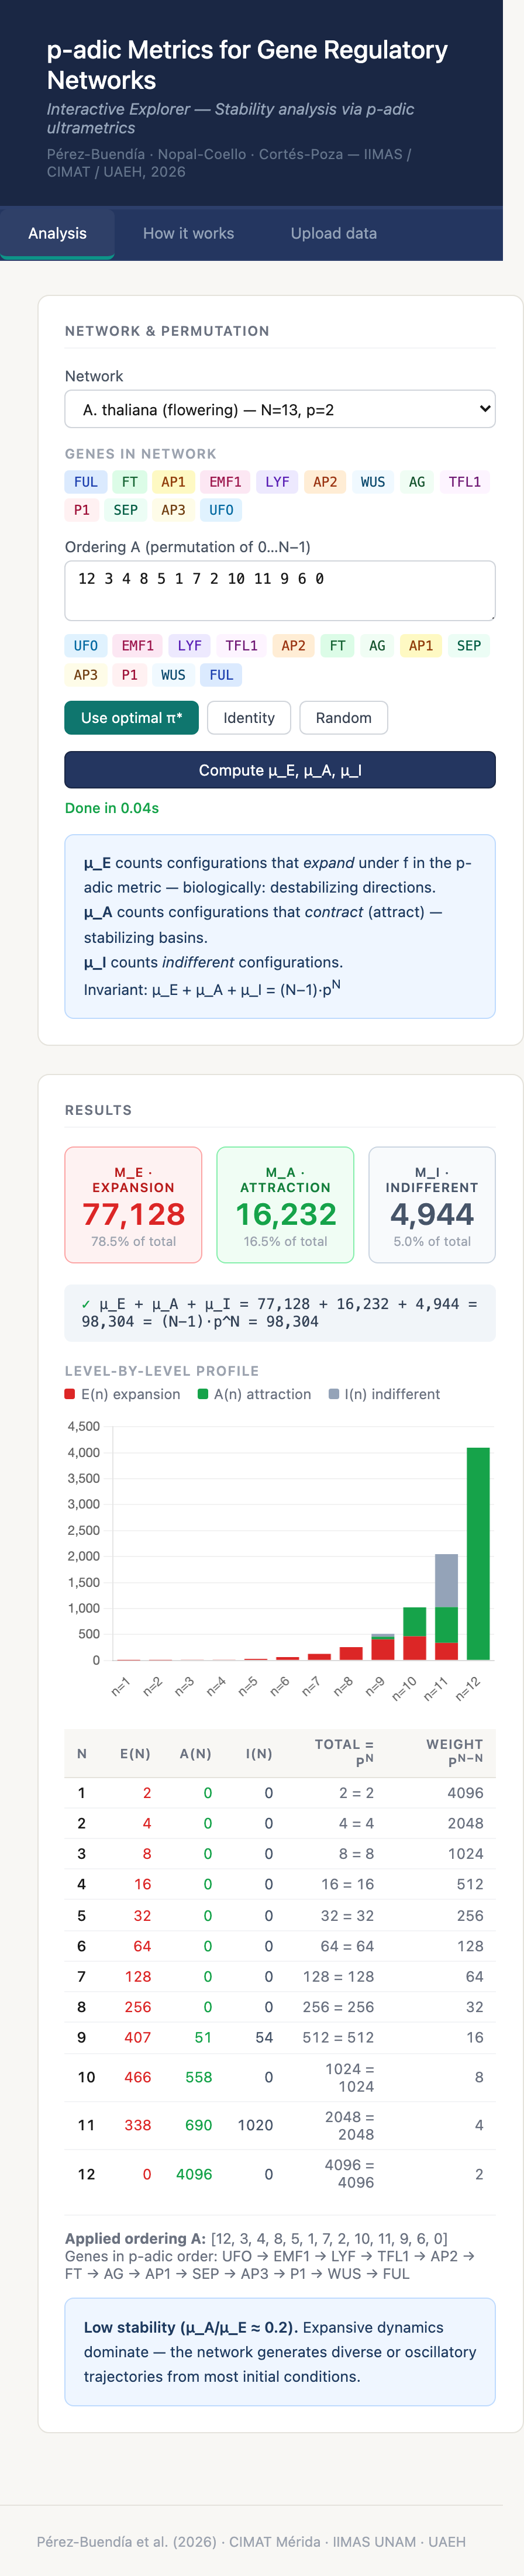
\includegraphics[width=0.47\textwidth,height=0.72\textheight,keepaspectratio]{web-demo-institucional/screenshots/registro-padic-grn-demo-running-mobile.png}
  \hfill
  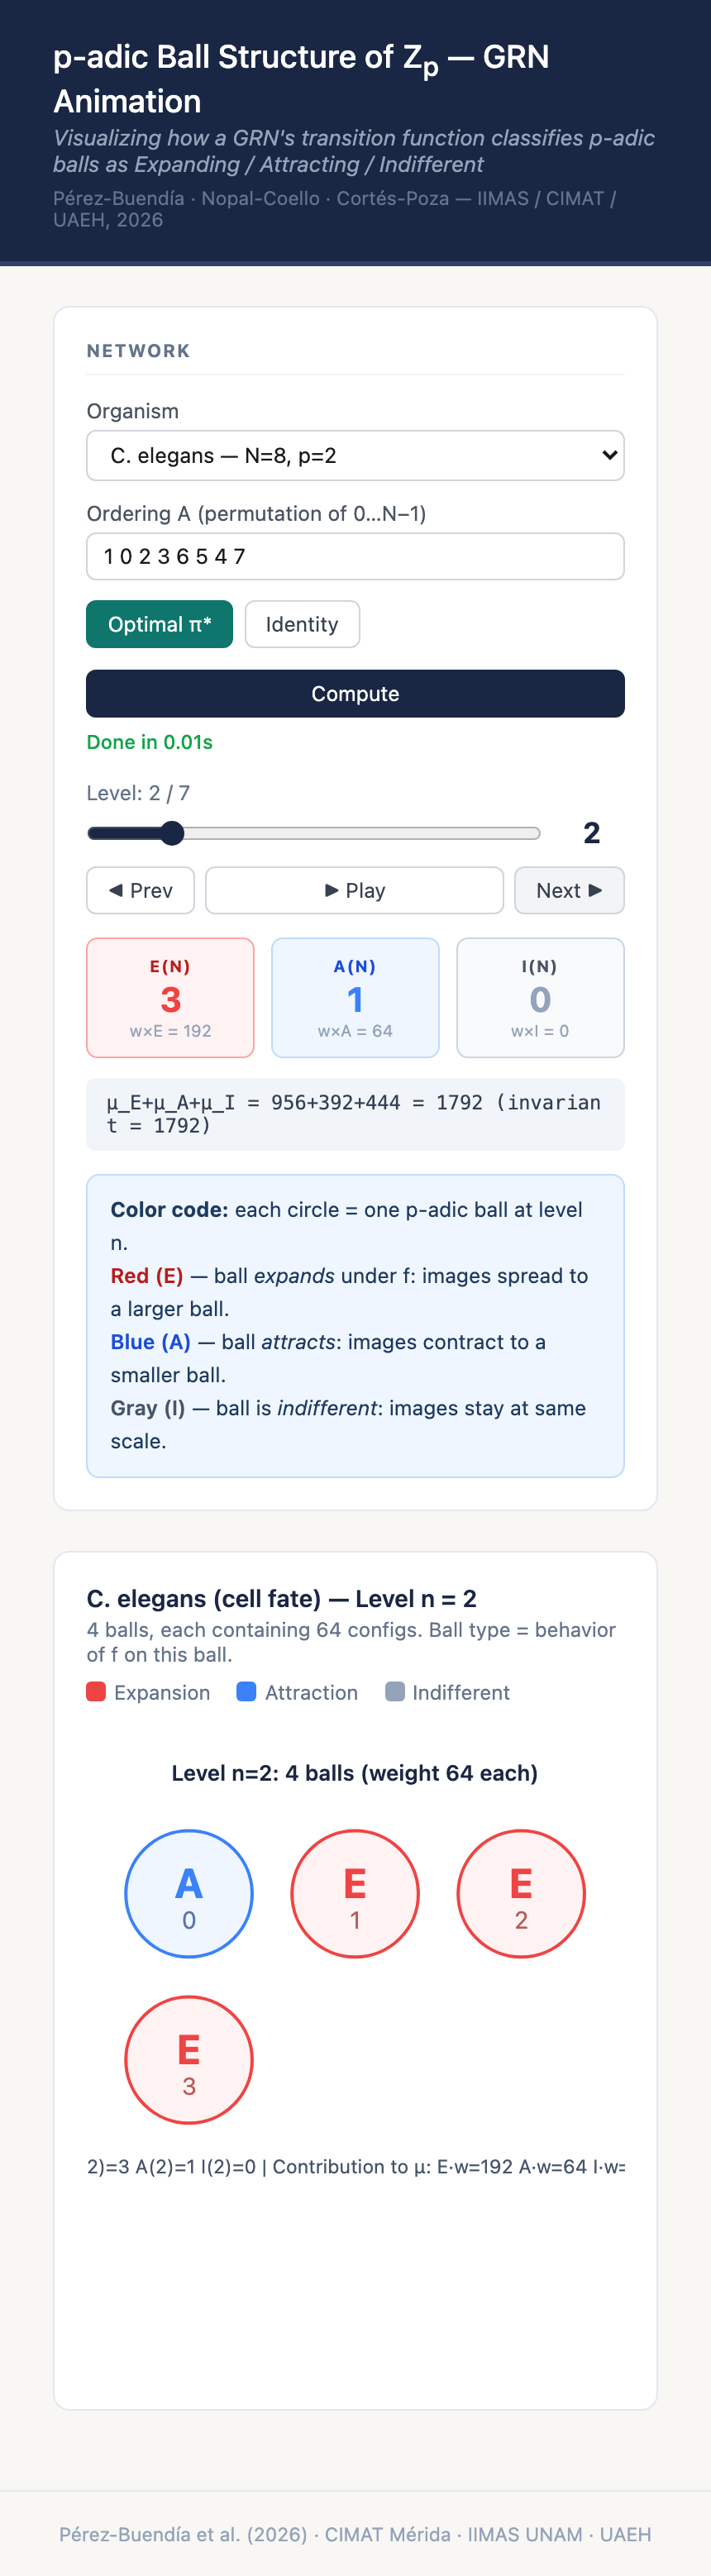
\includegraphics[width=0.47\textwidth,height=0.72\textheight,keepaspectratio]{web-demo-institucional/screenshots/registro-padic-balls-running-mobile.png}
  \caption{Ejecución móvil de los dos applets de análisis p-ádico con resultados y visualización activa.}
\end{figure}

\begin{figure}[htbp]
  \centering
  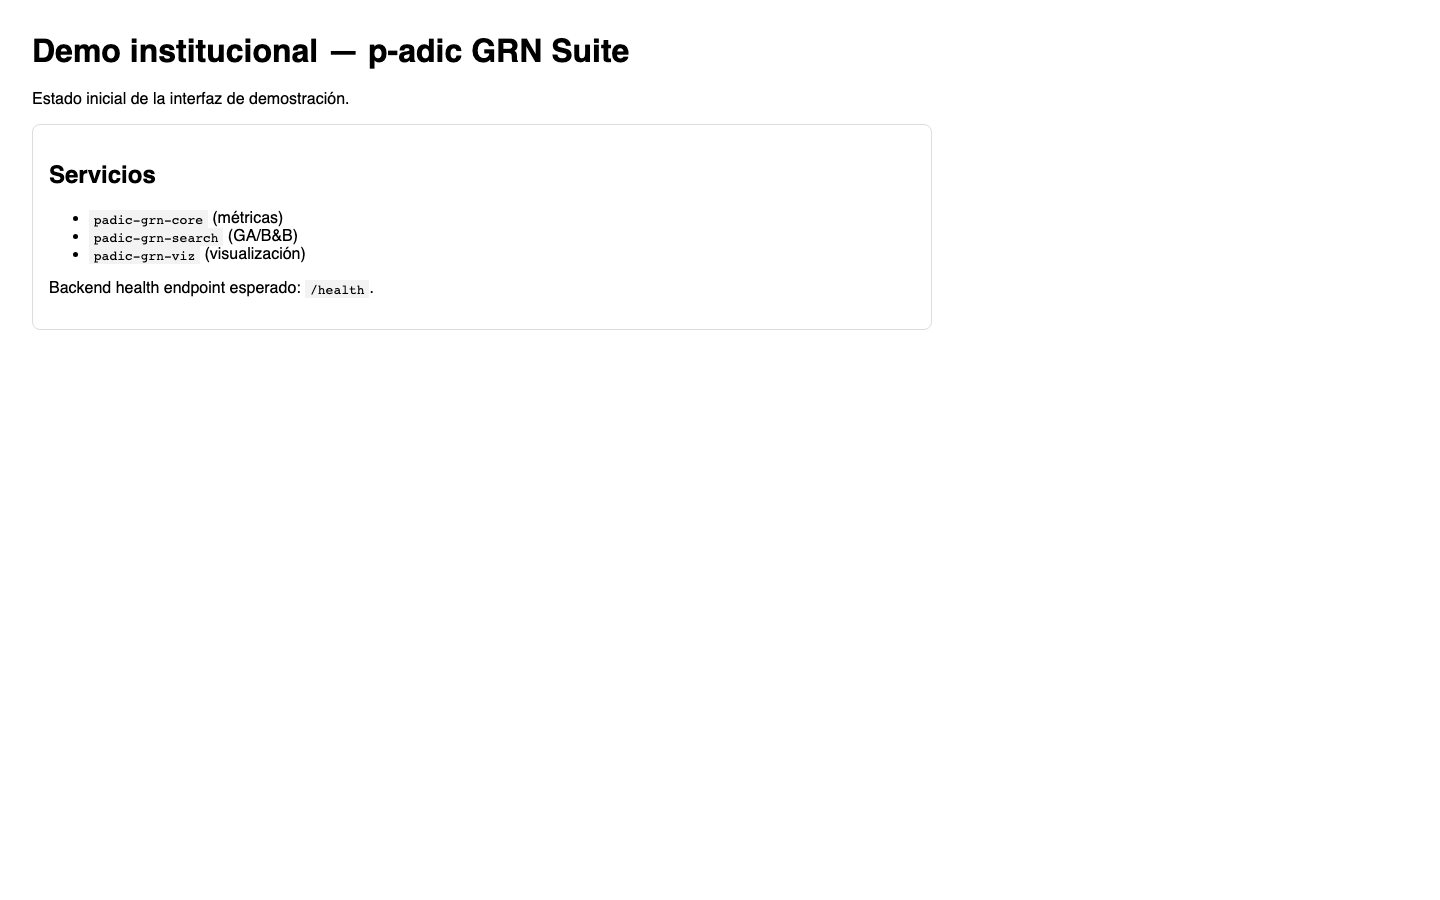
\includegraphics[width=\textwidth]{web-demo-institucional/screenshots/registro-frontend-index-desktop.png}
  \caption{Vista de portada del frontend institucional del demo web reportado.}
\end{figure}

\end{document}
